\section{The Approach}
\label{sec:framework}
In this section, we first propose a framework to evaluate the correlation of heterogeneous time series, and then we introduce how to use LSH scheme to do fast searching.

\subsection{Change Based Correlation Evaluation Framework}

The Change Based Correlation Coefficient can be calculated following the framework in Fig. \ref{fig:frame}.

\begin{description}
  \item[Step 1: Change Information Extraction] \hfill \\
  Given a time series, first, we extract the change information of the time series. 
  In this work, we regard the change information as bit-stream. In the bit-stream, $1$ denotes there is a change in this sub-series, and $0$ if not. 
  We will introduce the change based information extraction in details in the following section.
  \item[Step 2: Correlating Change Information] \hfill \\
  After obtaining the change information of the time series, we then calculate the correlation between the change information. In this work, we choose Jaccard similarity\cite{han2011data} coefficient to evaluate the correlation between change information.
\end{description}

In the rest of this section, we will introduce in detail of this framework.
%Given a time series, first, we extract the change information of the time series. 
%In this work, we regard the change information as bit-stream. In the bit-stream, $1$ denotes there is a change in this sub-series, and $0$ if not. We will introduce the change based information extraction in details in the following section.
%As we defined before (Section \ref{sec:formulation}), if two time series often change at the same time, they may have correlation with each other. 
%So, here, how often denotes the value of the correlation. In other words, how many $1$ do two time series both have. This is directly the Jaccard Distance.
%So, the Jaccard similarity between each bit-stream will be the correlation coefficient between these two time series. 


\begin{figure}[t]
\centering
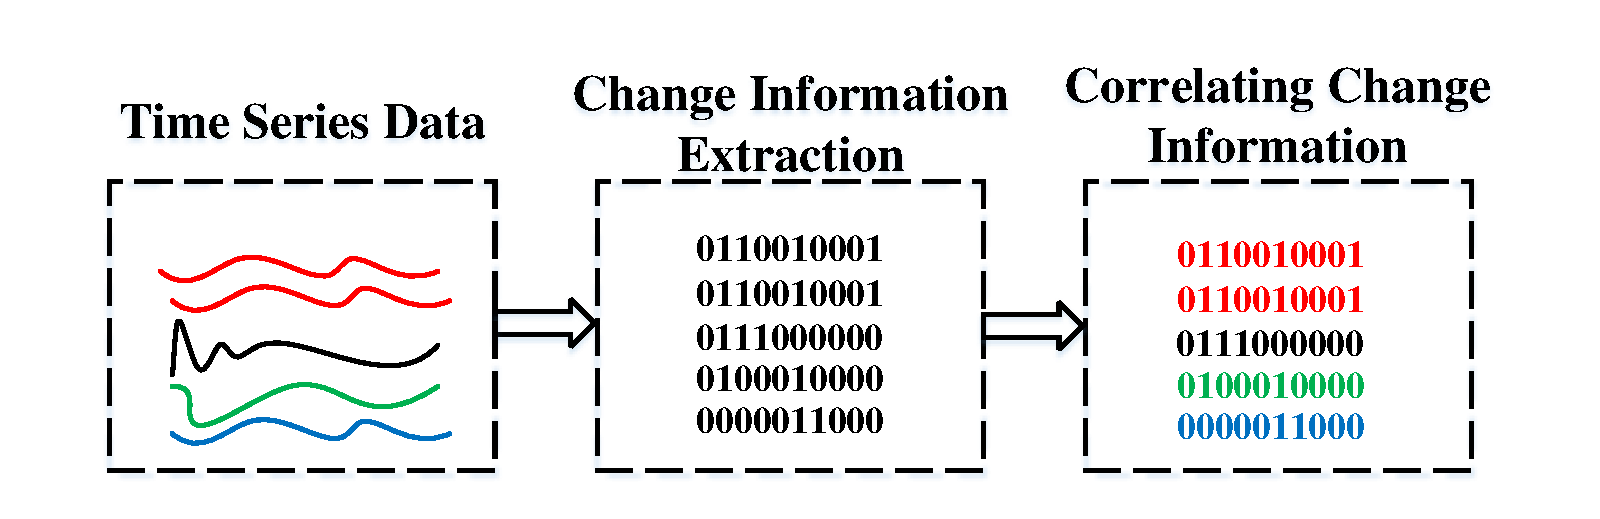
\includegraphics[width=0.5\textwidth]{framework.pdf}
\caption{Overview of the Framework}
\label{fig:frame}
\end{figure}

\subsection{Change Information Extraction}
\label{ChangeCorrelation}

As we introduced in Section.\ref{sec:formulation}, change based correlation corresponds to the change information of the time series. 
Change information of a time series is a time period information, not a time point information. 
As a result, in order to extract the change information of the time series, we need to find the information in small time period of the time series (A sub-series). 
The idea of extracting the change information is showed in Fig.\ref{fig:ChangeMapping}.

\begin{figure}[t]
\centering
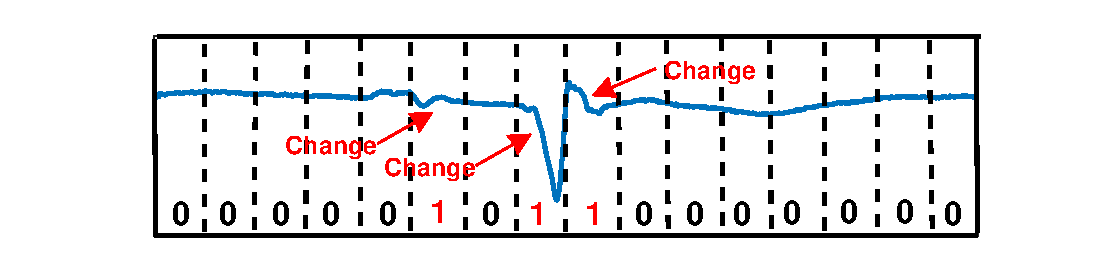
\includegraphics[width=0.5\textwidth]{changeExtraction.eps}
\caption{Change Information Extraction}
\label{fig:ChangeMapping}
\end{figure}

From Fig. \ref{fig:ChangeMapping} we can see, given a time series 
\[S = (s_1,s_2,...,s_m)\]
where $m$ is the number of points in the time series.
Given a subs-series length $w$, we divide the time series equally into $n = m/w$ equal pieces. It is pointed out that, $m/w$ may not be an integer, so in this work, we take the floor of $m/w$ as the value of $n$.
After dividing the time series equally into $n$ pieces, we can get a sub-series set , dented as follow
\[\Gamma_S = \{l_0,l_1,...,l_n\}\]
where, $l_i$ is the $i$th sub-series of $S$, and the formation of $l_i$ is showed as follow:
\[l_i = \{s_{i*w},s_{i*w+1},s_{i*w+2},...,s_{i*w+w-1}\}\]

Then the change information $b_i$ of each sub-series $l_i$ can be calculated as follow:

\begin{equation}
\label{Equ:ChangeInformation}
b_i = \left\{\begin{matrix}
1, & if~exist~change~in~l_i
\\ 
0, & if~without~change~in~l_i
\end{matrix}\right.
\end{equation}

Then, by using Equation \ref{Equ:ChangeInformation}, we can construct a bit-stream as follow:
\begin{equation}
\label{Equ:BitStream}
B_S = \{b_0,b_1,b_2,...,b_n\}
\end{equation}

We denote Equ.\ref{Equ:BitStream} as the change information of time series $S$. After getting this change information of time series $S$, we can then use it to calculate the correlation between different time series.

For the above discussion, we can find there are two key challenge for this change information extraction: (1) Given a sub-series $l_i$, how to denote whether there is a change in this sub-series, and (2) how to choose the sub-series length $w$.

In order to denote whether there's a change in the sub-series, we propose a change detection method to deal with this problem. On the other hand, we also discuss the sub-series length in our method.

\subsection{Change Detection in sub-series}
\label{sec:changeDetect}

As we introduced in previous section, after we divided the time series $S$ into small sub-series $l_i$, we need to detect whether there is a change in each sub-series $l_i$.

We formulate the problem as follow:

\begin{definition}[Change Detection]
Given a time series:
\[X = \{x_0,x_1,x_2,...,x_n\}\]
Denote whether there is a change in $X$.
\end{definition}
It is pointed out that, this problem is a binary classification problem, and the classification label is ``exist change" or ``without change".

In the result world, the change of a time series has three basic formations: 
\begin{itemize}
  \item \textbf{Frequency Change:} If the time series is a periodic time series and the frequency of the time series changes. 
  \item \textbf{Mean Change:} There is a mean shift happens in the time series.
  \item \textbf{Variance Change:} The variance of a time series changes.
\end{itemize}
We illustrate three different types of the time series in Fig. \ref{fig:ChangeType}.
And in this paper, we detect these three types of change individually, if there any of the change happens in this sub-series, we then say that there is a change in this sub-series.
\begin{figure}[t]
\centering
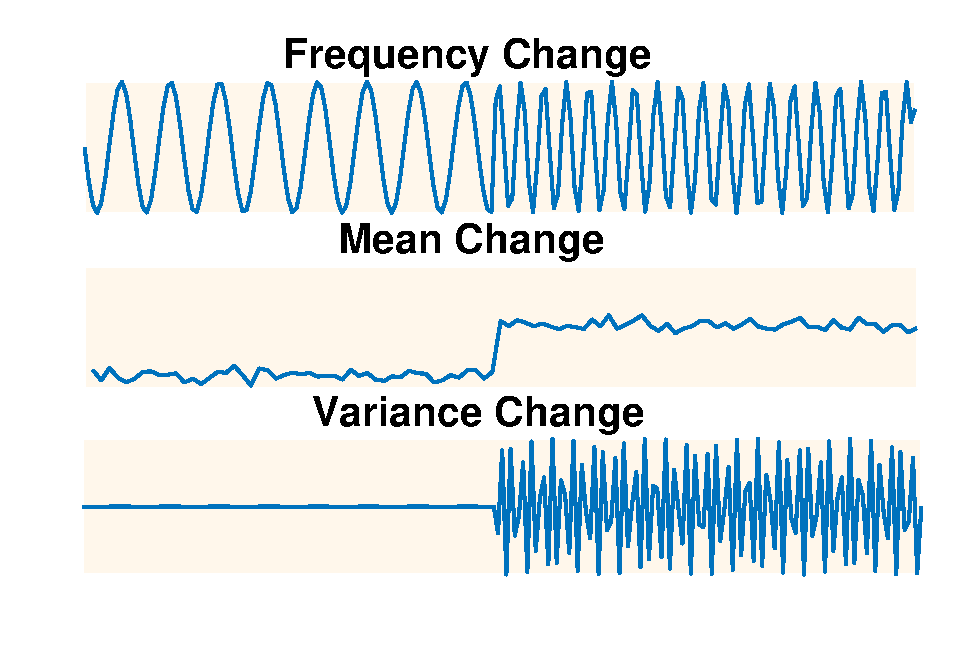
\includegraphics[width=0.5\textwidth]{ChangeType.eps}
\caption{Three different types of change: (1) Frequency Change, (2) Mean Change, and (3) Variance Change}
\label{fig:ChangeType}
\end{figure}

\subsubsection{Frequency Change Detection}

For a periodic time series, if there is a frequency change happens in this time series, then the there frequency must be multiple ($\geq 2 $) frequencies in this time series. In other words, if we can detect more than one frequency in this time series, there must be a frequency change happens.

In this work, we use Fourier transformation to detect the number of frequencies in a time series, Given a time series $X = \{x_0,x_1,x_2,...,x_n\}$, the discrete Fourier transformation (DFT) is showed as follow:

\begin{equation}
f_k = \sum_{t=0}^{n-1}x_t(\cos(-2\pi k\frac{t}{n})+i\sin(-2\pi \frac{t}{n}))
\end{equation}
where, $f_k$ denotes the amount of frequency $k$ in this time series. Then we can get a new time series $F$ denoted as follow:
\[ F = \{|f_1|,|f_2|,...,|f_{n/2}|\}\],
where $|f_i|$ denotes the absolute value of $f_k$. It is pointed out that, it is enough to only get a frequency domain series with length $n/2$, because the frequency domain series with length $n$ is a symmetric series, and the symmetric center is at $n/2$. Fig. \ref{fig:FFT} shows an example of the time domain of a time series and the frequency domain series.

\begin{figure}
\centering
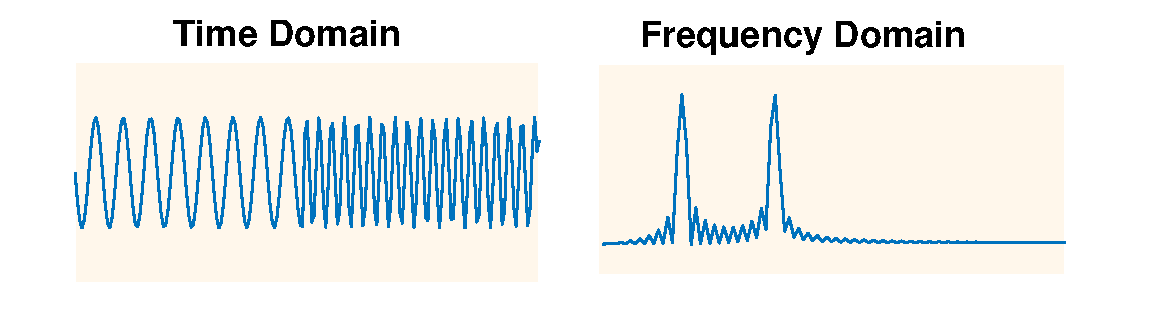
\includegraphics[width=0.5\textwidth]{FFT.eps}
\caption{Time domain of a time series and the frequency domain of the time series.}
\label{fig:FFT}
\end{figure}

After obtaining the frequency domain series, we just calculate the number huge peak of the frequency time series. If the number of huge peak is greater than $2$, then there is a change in this time series, otherwise, there is no change in this time series.

\subsubsection{Mean and Variance Change Detection}

In this work, we detect the change and variance change simultaneously.
Firstly, we equally divide the time series $X$ into two series: 
\[X_{f} = \{x_0,x_1,x_2,...,x_{n/2-1}\}\]
and, 
\[X_{r} = \{x_{n/2-1},x_{n/2},x_{n/2+1},...,x_{n-1}\}\]

Then, regard $X_{f}$ and $X_{r}$ as two data sampled from two distributions $P_1$ and $P_2$. So, if $P_1$ and $P_2$ are statistically the same, then we can say there's not change between each other. Otherwise, there is a change in this dataset. This idea comes from our previous research of detecting the correlation between event and time series.

Then, the problem here becomes a \textit{Two Sample Problem} \cite{gretton2006kernel}. We use the Two Sample \textit{t}-test \cite{moore2007basic} method to solve this problem:

Here, the $t_{score}$ between $X_{r}$ and $X_{r}$ can be calculated as:

\begin{equation}
t_{score} = \frac{\overline{X_{f}} - \overline{X_{r}}}{\sigma_p\sqrt{2/k}}
\end{equation}

where, $\overline{X_{f}}$ and $\overline{X_{r}}$ are the mean values of $X_{f}$ and $X_{r}$. And $\sigma_p$ is as follow:

\begin{equation}
\sigma_p = \frac{(k-1)\sigma_{X_{f}}^2 + (k-1)\sigma_{X_{r}}^2}{k-1}
\end{equation}

Then, if $t_{score} > \alpha$, we can say that these two samples are from different distributions, and thus there is a change in the sub-series $X$.

It is pointed out that, there are a so many time series change point detection methods \cite{liu2013change,chen2013contextual} proposed in the literature. 
All these change point detection methods can be used here to detect change information.
However, these algorithms are proposed to detect the change points rather than solve a binary classification problem. They can not exactly match our problem. We will review the change point detection algorithms in detail in Section. \ref{sec:relatedwork}.

\subsection{Discuss about Sub-series Length w}

In this research, the sub-series length $w$ is a very important parameter.
If the sub-series length $w$ is too small, then the change information can not be captured. 
On the other hand, if the sub-series length $w$ is too big, then there will be too much noise information.

In most of the cases, the value of $w$ can be selected based on domain knowledge and experiments. In the experiment of this work, all the sub-series length are selected based on the domain knowledge. 

However, in most real world problems, there are millions of time series and events, and we do not have enough domain knowledge to pre-select the values of all sub-series lengths. We need a method to automatically pre-assign the sub-series length.

In \cite{ding2015yading,luo2014correlating}, the authors proposed a method of find a sub-series length that can obtain as much as information and can have a shortest length to avoid noise.
Their method uses the first peak of the auto-correlation as their sub-series length.

Given a time series $S=(s_1,s_2,...,s_n)$, the autocorrelation is showed as follow:
\begin{equation}
R(l) = E(s_i*s_{i-l}).
\end{equation}
where $l$ denotes the lag of the correlation. The autocorrelation function of a time series can be used to represent the energy of signals in the time series with a period of $l$ \cite{hamilton1994time}. Therefore, our length $w$ can be assigned as the value of the first peak to include the significant signal of the time series. For more detail of this selection method, please refer \cite{luo2014correlating,ding2015yading}.

\subsection{Jaccard Similarity Coefficient}

After obtaining the change information (Bit-stream) of each data, we then use Jacord Similarity Coefficient to calculate the Change Correlation of each time series.

The Jaccard Similarity \cite{han2011data} is defined as follow:
Given two Bit-stream $X$ and $Y$, the Jaccord distance is showed as follow:

\begin{equation}
J(A,B) = \frac{|A \cap B|}{|A \cup B|}
\end{equation}

where, $|A \cap B|$ denotes the number of bit that $X$ and $Y$ both $1$. And $|A \cup B|$ denotes the number of bit that at least $X$ or $Y$ is $1$.
For example, given two bit stream: $X={100111}$, and $Y={001110}$. Then $|A \cap B| = 2$, and $|A \cap B| = 5$, so $J(A,B) = \frac{2}{5} = 0.4$.

\subsection{LSH Scheme}

In many the real world problems, the scale of time series data often huge \cite{rakthanmanon2012searching}. Mining such huge number of time series is a big challenge for us.

In this work, the change information of a time series is a bit-stream (Equ. \ref{Equ:BitStream}). 
We regard it as the hashing code of the original time series. 
This admit us to use locality sensitive hashing scheme to do fast search and mining.
For example, in this work, we use minhash to do fast top-k search. Due to the page limitation of this paper, we do not introduce the detailed steps of LSH search. If you interested in this part, please refer \cite{shrivastava2014asymmetric,indyk1998approximate}.

\subsection{Correctness Discussion}

In this subsection, we briefly discuss about the reason that the proposed framework can correctly evaluate the correlation defined in Section.\ref{sec:relatedwork} Equation. \ref{def:changeCorrelaion}.

The proposed framework can detect change based correlation because of the following reasons:

\begin{itemize}
  \item Recall the definition of time stamps showed in Section \ref{sec:formulation}, the equality of two time stamp is defined within a toleration of a small time interval $\sigma$. In other world, the change point in such small interval can be regarded as the same change. 
  As a result, the if two time series both have change point at this small interval, that means  these two time series have the same change point.
  So, the change information extraction can obtain all the change point information of the time series.
  \item The Jaccard Similarity Coefficient used in our method just match the jaccard distance in the change based correlation coefficient.
\end{itemize}

As a result, because of the above reasons, the proposed framework can correctly detect the correlation defined in Equation.\ref{def:changeCorrelaion}.
